\section{Introduction}
\begin{frame}{Introduction}{}
\begin{block}{Standard \emph{shapes} of information security:}
	\begin{itemize}
		\item Confidentiality
		\item Integrity
		\item Availability
	\end{itemize}
\end{block}
\begin{quote}
	There is a new security that we want to obtain: \textbf{Anonymity}
	Anonymity [...] means that the personal identity,
	or personally identifiable information of that person is not known.
\end{quote}
\end{frame}

\begin{frame}{Introduction}{anonymity methods}
There are a lot of anonymity driven software online, like \textit{i2p},
\textit{freenet} or \textit{Tor}, we will talk about the last one because
is the most used and expanded in the real world
(2 million of client per day!).
\end{frame}

\begin{frame}{Onion Routing}{}
The onion routing model is a way to gain anonymity on the net:
\begin{itemize}
	\item Provides anonymity
	\item Protects from sniffing
\end{itemize}
Introduced by David Goldshlag, Paul Syverson and Michael Reed in the 1999.
\\
It recalls an onion because every step \textbf{peel} a layer.
\\
Let us see an implementation.
\end{frame}

\begin{frame}{Tor}{The onion router}
\begin{block}{Overview}
Tor is a group of volunteers that operates to defend anonymity online.\\
The system is based on an interconnection of machines, called \textbf{routers}.\\
It operates over the network level 4.
\end{block}
It operates as follow:
\end{frame}

\begin{frame}{Tor}{Tor workings}
\begin{center}
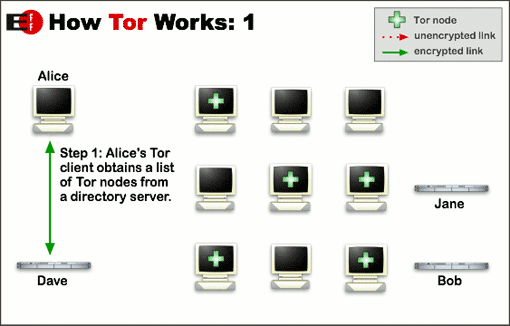
\includegraphics[scale=0.54]{img/tor1.png}
\end{center}
\end{frame}

\begin{frame}{Tor}{Tor workings}
\begin{center}
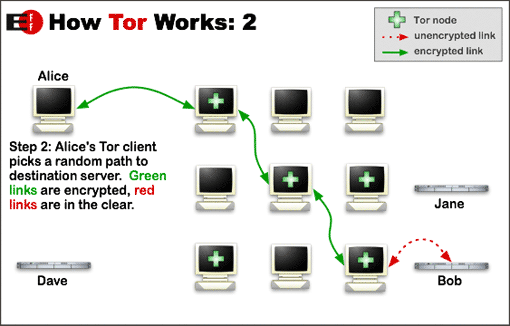
\includegraphics[scale=0.54]{img/tor2.png}
\end{center}
\end{frame}

\begin{frame}{Tor}{Tor workings}
\begin{center}
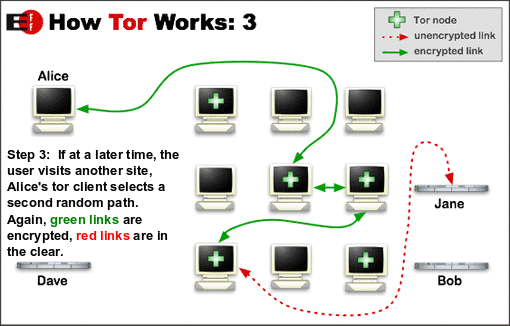
\includegraphics[scale=0.72]{img/tor3.png}
\end{center}
\end{frame}

\begin{frame}{Tor}{Tor encryption}
\begin{center}
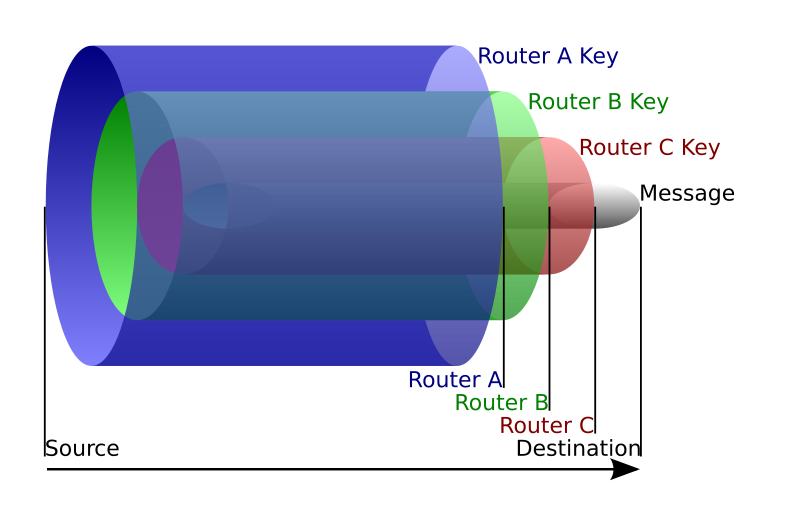
\includegraphics[scale=0.35]{img/onion.png}
\end{center}
\end{frame}

\subsection{Attacks}
\begin{frame}
\end{frame}
\section{Simulation}
\subsection{Shadow}
\subsection{Plug-ins}
